\documentclass[a4paper]{book}
\usepackage[left=2.00cm, right=2.00cm, top=2.50cm, bottom=2.00cm]{geometry}

\usepackage{amsmath,amssymb}
\usepackage{graphicx}
\usepackage{color}
\definecolor{bl}{gray}{0.9}

% figure position
\usepackage{booktabs}
\usepackage{here}

\title{Note: The Elements of Computing Systems}

\begin{document}
\maketitle

\chapter*{Preface}
This is my study note for The Elements of Computing Systems (ISBN:  978-0262640688) by Noam Nisan and Shimon Schocken.

\chapter{Boolean Logic}
\textbf{Boolean Algebra}
\begin{align*}
    x ~\mathrm{or}~ y & = \bar{x}y + x\bar{y} + xy \\
    &                   = \bar{x}y + x(y + \bar{y}) \\
    &                   = x + \bar{x}y \\
    &                   = x + \overline{ x + \bar{y} } \\
    &                   = \overline{ \overline{ x + \overline{(x + y) } } } \\
    &                   = \overline{\bar{x} (x + \bar{y} ) } \text{~ ~ ~ where } \overline{x + y} = \bar{x} \bar{y} \\
    &                   = \overline{ x\bar{x} + \bar{x}\bar{y} } \\
    &                   = \overline{ \bar{x} \bar{y} } \\
    &                   = \overline{\overline{x + y}} \\
    &                   = x + y \\
%
%
    \text{if } y \text{ then } x & = \bar{x}\bar{y} + x \bar{y} + xy \\
    &                              = \bar{x}\bar{y} + x(y + \bar{y}) \\
    &                              = x + \bar{x}\bar{y} \\
    &                              = x + \overline{x + y} \\
    &                              = \overline{ \overline{ x + \overline{x + y} } } \\
    &                              = \overline{ \bar{x}(x + y) } \\
    &                              = \overline{ x\bar{x} + \bar{x}y } \\
    &                              = \overline{ \bar{x}y } \\
    &                              = x + \bar{y} \\
%
%
    \text{if } x \text{ then } y & = \bar{x}\bar{y} + \bar{x}y + xy \\
    &                              = \bar{x}\bar{y} + (x + \bar{x}) y \\
    &                              = \bar{x}\bar{y} + y \\
    &                              = \overline{x + y} + y \\
    &                              = \overline{ \overline{ \overline{x + y} + y} } \\
    &                              = \overline{ (x + y) \bar{y} } \\
    &                              = \overline{ x\bar{y} + y\bar{y} } \\
    &                              = \overline{ x \bar{y} } \\
    &                              = \bar{x} + y \\
%
%
    x \text{ nand } y & = \bar{x}\bar{y} + \bar{x}y + x \bar{y} \\
    &                   = \bar{y}(x + \bar{x}) + \bar{x} y \\
    &                   = \bar{y} + \bar{x} y \\
    &                   = \bar{x} + \bar{y} \text{~ ~ ~ where } x + y    = x + \bar{x}y \\
    &                   = \overline{ \overline{ \bar{x} + \bar{y} } } \\
    &                   = \overline{ xy }
\end{align*}







\setcounter{chapter}{4}
%%%%%%%%%%%%%%%%%%%%%%%%%%%%%%%%%%%%%%%%%%%%
%%%%%%%%%%%%%%%%%%%%%%%%%%%%%%%%%%%%%%%%%%%%
\chapter{Computer Architecture}




\section{Memory}
\begin{figure}[H]
    \centering
    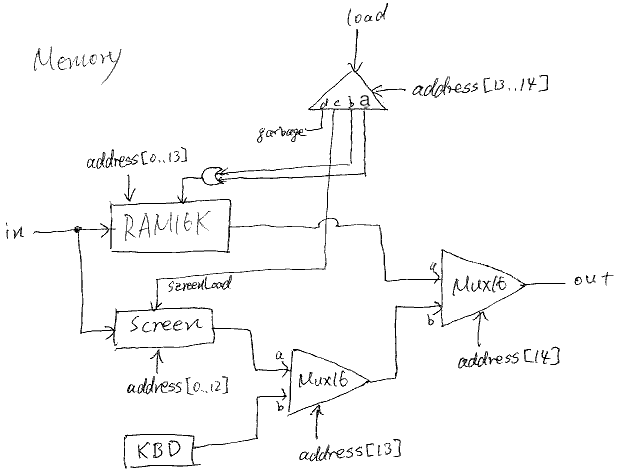
\includegraphics{pic/project05/memory.png}
    \caption{memory}
\end{figure}


\section{CPU}

$\text{C-instruction} = 111a c_1 c_2 c_3 c_4 c_5 c_6 d_1 d_2 d_3 j_1 j_2 j_3$

\begin{itemize}
    \item $d_1$: destination A
    \item $d_2$: destination D
    \item $d_3$: destination M
\end{itemize}


\begin{figure}[H]
    \centering
    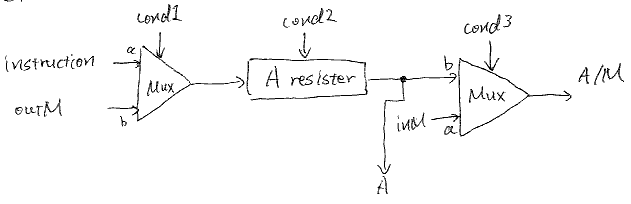
\includegraphics{pic/project05/cpu1.png}
    \caption{memory}
\end{figure}

\begin{align*}
    \text{cond1} & = \text{instruction}[15] \\
    \text{cond2} & = (\text{not } \text{instruction}[15]) \text{ or } (\text{instruction}[15] \text{ and } \text{instruction}[5]) \\
    \text{cond3} & = \text{instruction}[15] \text{ and } \text{ not } \text{instruction}[12]
\end{align*}

\begin{itemize}
    \item instruction[15]: opcode
    \item instruction[12]: C-instruction's $a$. If $a$ is $1$, comp includes A, otherwise, comp includes M.
    \item instruction[5]: destination A.
\end{itemize}


\begin{figure}[H]
    \centering
    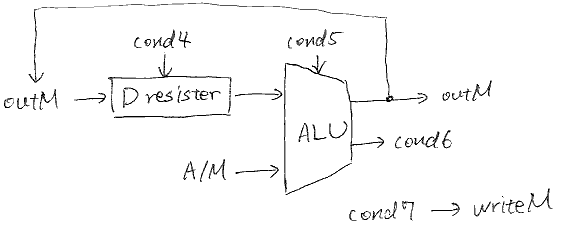
\includegraphics{pic/project05/cpu2.png}
    \caption{memory}
\end{figure}

\begin{align*}
    \text{cond4} & = \text{instruction}[15] \text{ and } \text{instruction}[4] \\
    \text{cond5} & = \begin{cases}
                        \text{zx} = \text{instruction}[11] = c_1 \\
                        \text{nx} = \text{instruction}[10] = c_2 \\
                        \text{zy} = \text{instruction}[9] = c_3 \\
                        \text{ny} = \text{instruction}[8] = c_4 \\
                        \text{f}  = \text{instruction}[7] = c_5 \\
                        \text{no} = \text{instruction}[6] = c_6
                    \end{cases} \\
    \text{cond6} & = (\text{zr}, \text{ng}) \\
    \text{cond7} & = \text{instruction}[15] \text{ and } \text{instruction}[3]
\end{align*}

\begin{itemize}
    \item \text{instruction}[3]: $d_3$, destination M
    \item \text{instruction}[4]: $d_2$, destination D
\end{itemize}



\begin{figure}[H]
    \centering
    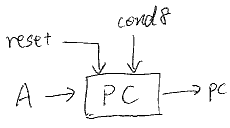
\includegraphics{pic/project05/cpu3.png}
    \caption{memory}
\end{figure}


\begin{align*}
    \text{cond8} = & \overline{\text{zr}} \cdot \overline{\text{ng}} \cdot \overline{j_1} \cdot \overline{j_2} \cdot \overline{j_3} \text{~~~~~~~ (JGT)} \\
                 & + \overline{\text{zr}} \cdot \overline{j_1} \cdot j_2 \cdot j_3 \text{~~~~~~ (JEQ)} \\
                 & + \overline{\text{ng}} \cdot \overline{j_1} \cdot j_2 \cdot j_3 \text{~~~~~~ (JGE)} \\
                 & + \text{ng} \cdot j_1 \cdot \overline{j_2} \cdot \overline{j_3} \text{~~~~~~ (JLT)} \\
                 & + \overline{\text{zr}} \cdot j_1 \cdot \overline{j_2} \cdot j_3 \text{~~~~~~ (JNE)} \\
                 & + (\text{zr} + \text{ng}) \cdot j_1 \cdot j_2 \cdot \overline{j_3} \text{~~~~~~ (JLE)} \\
                 & + j_1 \cdot j_2 \cdot j_3 \text{~~~~~~ (JMP)}
\end{align*}

\setcounter{chapter}{6}
\chapter{Virtual Machine I: Stack Arithmetic}
\section{Arithmetic}

\[
    \texttt{add (sub)}
    \Rightarrow
    %
    \begin{cases}
        \texttt{ // SP--                            } \\
        \texttt{ @SP                                } \\
        \texttt{ M=M-1                              } \\
        \\
        \texttt{ // D = y                           } \\
        \texttt{ A=M                                } \\
        \texttt{ D=M                                } \\
        \\
        \texttt{ // SP--                            } \\
        \texttt{ @SP                                } \\
        \texttt{ M=M-1                              } \\
        \\
        \texttt{ // *SP = y + x (add) / x - y (sub) } \\
        \texttt{ A=M                                } \\
        \texttt{ M=D+M (add) / M=M-D (sub)          } \\
        \\
        \texttt{ // SP++                            } \\
        \texttt{ @SP                                } \\
        \texttt{ M=M+1                              }
    \end{cases}
\]

\[
    \texttt{neg, not}
    \Rightarrow
    %
    \begin{cases}
        \texttt{ // SP--                 } \\
        \texttt{ @SP                     } \\
        \texttt{ @M=M-1                  } \\
        \\
        \texttt{ // -M                   } \\
        \texttt{ A=M                     } \\
        \texttt{ M=-M (neg) / M=!M (not) } \\
        \\
        \texttt{ // SP++                 } \\
        \texttt{ @SP                     } \\
        \texttt{ M=M+1                   }
    \end{cases}
\]


\[
    \texttt{eq, gt, lt}
    \Rightarrow
    \begin{cases}
        ~ ~ ~ ~\texttt{ // SP--                             } \\
        ~ ~ ~ ~\texttt{ @SP                                 } \\
        ~ ~ ~ ~\texttt{ M=M-1                               } \\
        ~ ~ ~ ~\\
        ~ ~ ~ ~\texttt{ // D = y                            } \\
        ~ ~ ~ ~\texttt{ D=M                                 } \\
        ~ ~ ~ ~\\
        ~ ~ ~ ~\texttt{ // SP--                             } \\
        ~ ~ ~ ~\texttt{ @SP                                 } \\
        ~ ~ ~ ~\texttt{ M=M-1                               } \\
        ~ ~ ~ ~\\
        ~ ~ ~ ~\texttt{ // x - y                            } \\
        ~ ~ ~ ~\texttt{ A = M                               } \\
        ~ ~ ~ ~\texttt{ D=M-D                               } \\
        ~ ~ ~ ~\\
        ~ ~ ~ ~\texttt{ // if condition then -1 else 0 end  } \\
        ~ ~ ~ ~\texttt{ @then                               } \\
        ~ ~ ~ ~\texttt{ D;jEQ (eq),  D;JGT (gt), D:JLT (lt) } \\
        ~ ~ ~ ~\texttt{ @SP                                 } \\
        ~ ~ ~ ~\texttt{ A=M                                 } \\
        ~ ~ ~ ~\texttt{ M=0                                 } \\
        ~ ~ ~ ~\texttt{ @end                                } \\
        ~ ~ ~ ~\texttt{ 0;JMP                               } \\
        \texttt{ (then)                                     } \\
        ~ ~ ~ ~\texttt{ @SP                                 } \\
        ~ ~ ~ ~\texttt{ A=M                                 } \\
        ~ ~ ~ ~\texttt{ M=-1                                } \\
        \texttt{ (end)                                      } \\
        \\
        ~ ~ ~ ~\texttt{ // SP++                             } \\
        ~ ~ ~ ~\texttt{ @SP                                 } \\
        ~ ~ ~ ~\texttt{ M=M+1                               } \\
    \end{cases}
\]

\[
    \texttt{and, or}
    \Rightarrow
    \begin{cases}
        \texttt{ // SP++       } \\
        \texttt{ @SP           } \\
        \texttt{ M=M-1         } \\
        \\
        \texttt{ // D = y      } \\
        \texttt{ A=M           } \\
        \texttt{ D=M           } \\
        \\
        \texttt{ // SP--       } \\
        \texttt{ @SP           } \\
        \texttt{ M=M-1         } \\
        \\
        \texttt{ // *SP = y\&x } \\
        \texttt{ A=M           } \\
        \texttt{ M=D\&M        } \\
        \\
        \texttt{ // SP++       } \\
        \texttt{ @SP           } \\
        \texttt{ M=M+1         }
    \end{cases}
\]


\section{logical command}
% push constant i
\[
    \texttt{push constant i}
    \Rightarrow
    %
    \begin{cases}
        \texttt{*SP = i} \\
        \texttt{SP++}
    \end{cases}
    %
    \Rightarrow
    %
    \begin{cases}
        \texttt{// *SP=i} \\
        \texttt{@i} \\
        \texttt{D=A} \\
        \texttt{@SP} \\
        \texttt{A=M} \\
        \texttt{M=D} \\
        \\
        \texttt{// SP++} \\
        \texttt{@SP} \\
        \texttt{M=M+1}
    \end{cases}
\]


% push segment i: segment = {local, argument, this that}
\[
    \texttt{push segment i}
    \Rightarrow
    %
    \begin{cases}
        \texttt{addr =  SEG + i } \\
        \texttt{*SP = *addr     } \\
        \texttt{SP++            }
    \end{cases}
    %
    \Rightarrow
    %
    \begin{cases}
        \texttt{// addr = SEG + i } \\
        \texttt{@SEG              } \\
        \texttt{D=M               } \\
        \texttt{@i                } \\
        \texttt{A=D+A             } \\
        %
        \\
        \texttt{// *addr          } \\
        \texttt{D=M               } \\
        \\
        \texttt{// *SP = *addr    } \\
        \texttt{@SP               } \\
        \texttt{A=M               } \\
        \texttt{M=D               } \\
        %
        \\
        \texttt{// SP++           } \\
        \texttt{@SP               } \\
        \texttt{M=M+1             }
    \end{cases}
\]
where \texttt{segment = local, argument, this, that}.

\[
    \texttt{push pointer i}
    \Rightarrow
    \begin{cases}
        \texttt{ @THIS // or @R3 } \\
        \texttt{ D=M             } \\
        \texttt{ @i              } \\
        \texttt{ A=D+A           } \\
        \texttt{ D=M             } \\
        \texttt{ @SP             } \\
        \texttt{ A=M             } \\
        \texttt{ M=D             } \\
        \texttt{ @SP             } \\
        \texttt{ M=M+1           }
    \end{cases}
\]


\[
    \texttt{push static i}
    \Rightarrow
    \begin{cases}
        \texttt{ @Xxx.i } \\
        \texttt{ D=M    } \\
        \texttt{ @SP    } \\
        \texttt{ A=M    } \\
        \texttt{ M=D    } \\
        \texttt{ @SP    } \\
        \texttt{ M=M+1  }
    \end{cases}
\]
where this vm program name is \texttt{Xxx.vm}.

% pop segment i
\[
    \texttt{pop segment i}
    \Rightarrow
    %
    \begin{cases}
        \texttt{addr = SEG + i } \\
        \texttt{SP--           } \\
        \texttt{*addr = *SP    }
    \end{cases}
    %
    \Rightarrow
    %
    \begin{cases}
        \texttt{SEG = SEG + i } \\
        \texttt{SP--          } \\
        \texttt{*SEG = *SP    } \\
        \texttt{SEG = SEG - i }
    \end{cases}
    %
    \Rightarrow
    %
    \begin{cases}
        \texttt{// SEG=SEG+i  } \\
        \texttt{@SEG          } \\
        \texttt{D=M           } \\
        \texttt{@i            } \\
        \texttt{D=D+A         } \\
        \texttt{@SEG          } \\
        \texttt{M=D           } \\
        \\
        \texttt{// SP--       } \\
        \texttt{@SP           } \\
        \texttt{M=M-1         } \\
        \\
        \texttt{// *SP        } \\
        \texttt{A=M           } \\
        \texttt{D=M           } \\
        \\
        \texttt{// *SEG = *SP } \\
        \texttt{@SEG          } \\
        \texttt{A=M           } \\
        \texttt{M=D           } \\
        \\
        \texttt{// SEG=SEG-i  } \\
        \texttt{@i            } \\
        \texttt{D=A           } \\
        \texttt{@SEG          } \\
        \texttt{M=M-D         } \\
    \end{cases}
\]
where \texttt{segment = local, argument, this, that}.

\texttt{\colorbox{bl}{pop pointer i}} is equivalent to \texttt{\colorbox{bl}{pop this i}} where $i = 0, 1$.


\[
    \texttt{pop static i}
    \Rightarrow
    \begin{cases}
        \texttt{ // SP-- } \\
        \texttt{ @SP     } \\
        \texttt{ M=M-1   } \\
        \\
        \texttt{ // *SP  } \\
        \texttt{ A=M     } \\
        \texttt{ D=M     } \\
        \\
        \texttt{ @Xxx.i  } \\
        \texttt{ M=D     }
    \end{cases}
\]
\end{document}
